
%(BEGIN_QUESTION)
% Copyright 2006, Tony R. Kuphaldt, released under the Creative Commons Attribution License (v 1.0)
% This means you may do almost anything with this work of mine, so long as you give me proper credit

Koble følgende operasjonsforsterkerkretser til riktig overføringsfunksjon fra listen under (merk at det er listet opp mer enn seks funksjoner, bare for å gjøre oppgaven litt mer utfordrende):

$$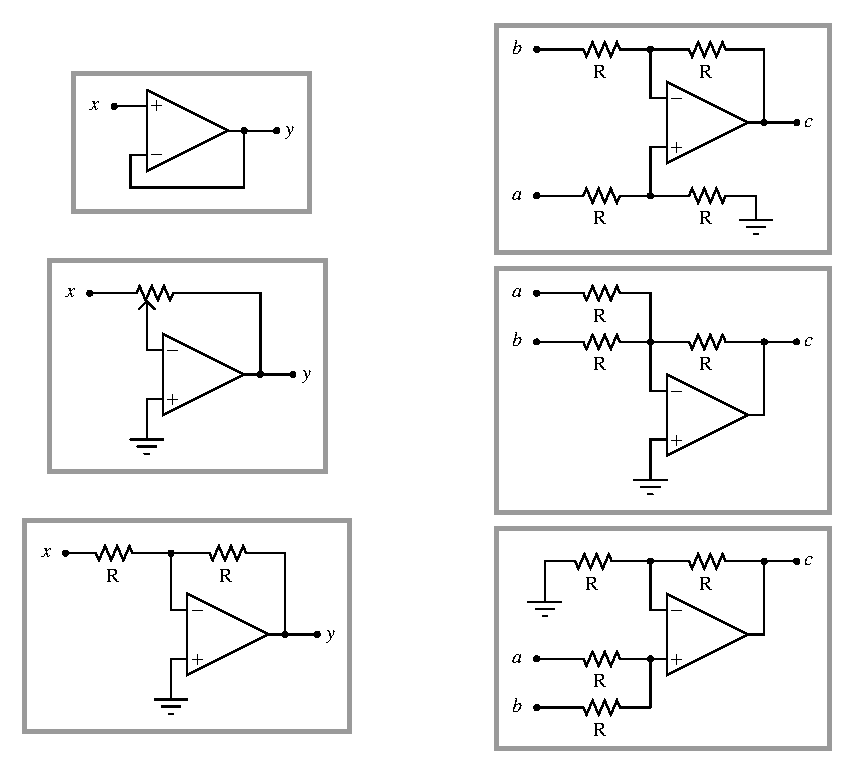
\includegraphics[width=15.5cm]{i01466x01.eps}$$

Merk: Alle motstandene merket $R$ har nøyaktig samme verdi. $k$ som vises i noen av ligningene representerer en ``programmerbar'' konstant:

\vskip 10pt

$y = -kx$ \hskip 50pt $c = -(a + b)$ \hskip 50pt $y = 2x$ \hskip 50pt $y = x$ \hskip 50pt $y = -x$ 

\vskip 10pt

$c = a + b$ \hskip 50pt $y = kx$ \hskip 70pt $c = 2(a + b)$ \hskip 30pt $y = x \div k$ \hskip 30pt $c = a - b$ 

\vskip 20pt \vbox{\hrule \hbox{\strut \vrule{} {\bf Forslag til sokratisk diskusjon} \vrule} \hrule}

\begin{itemize}
\item{} Identifiser ``forenklende antakelser'' som vi vanligvis bruker når vi analyserer DC-opampkretser. Tips: Én handler om virkningen av negativ tilbakekobling på inngangsspenningene, og en annen handler om strøm i inngangsterminalene.
\item{} Forklar {\bf hvorfor} hver krets utfører sin respektive matematiske funksjon.
\item{} Forklar hvor fortegn minus kommer fra i noen av kretsligningene.
\end{itemize}

\underbar{file i01466}
%(END_QUESTION)





%(BEGIN_ANSWER)

$$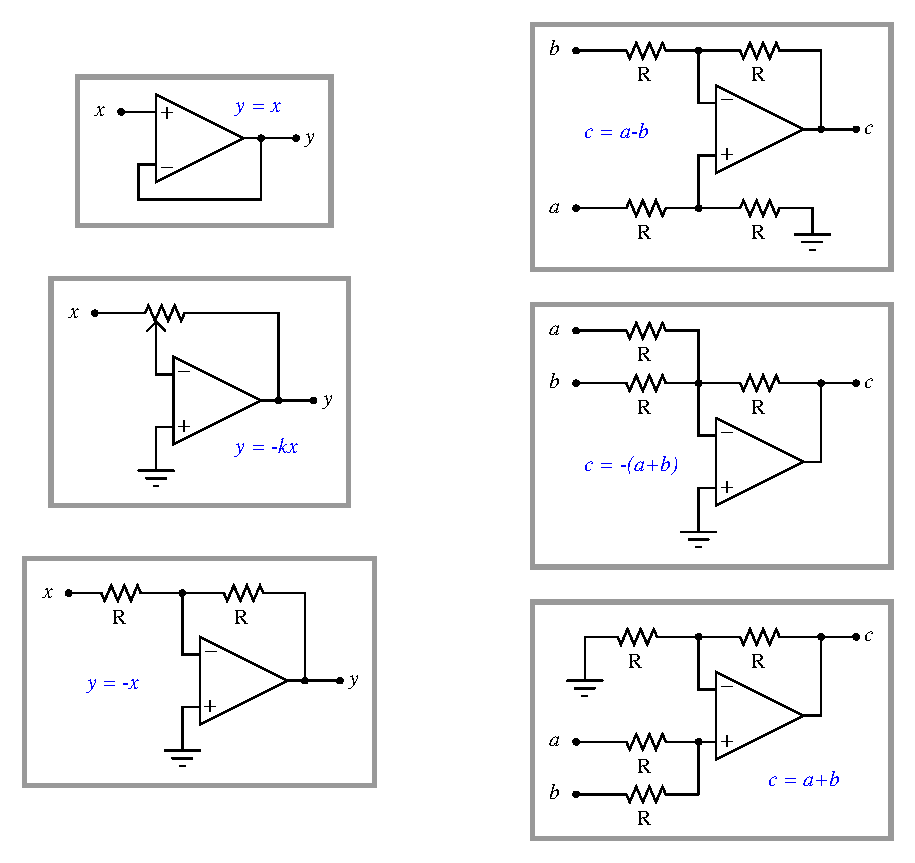
\includegraphics[width=15.5cm]{i01466x02.eps}$$

%(END_ANSWER)





%(BEGIN_NOTES)



%INDEX% Electronics review: opamp ``function blocks''

%(END_NOTES)
